\documentclass[]{spie}  %>>> use for US letter paper
%\documentclass[a4paper]{spie}  %>>> use this instead for A4 paper
%\documentclass[nocompress]{spie}  %>>> to avoid compression of citations

\renewcommand{\baselinestretch}{1.0} % Change to 1.65 for double spacing
 
\usepackage{amsmath,amsfonts,amssymb}
\usepackage{graphicx}
\usepackage[colorlinks=true, allcolors=blue]{hyperref}
\usepackage{glossaries}
\usepackage{caption}

\usepackage{subcaption}
\title{Simulating the Effects of Exozodiacal Dust in WFIRST CGI observations}

\author[a]{Ewan S. Douglas}
\author[b]{John Debes}
\author[a]{Kian Miliani}
\author[b]{Bin Ren}
\author[c]{Yinzi Xin}
\author[c]{Kerri L. Cahoy}
\author[d]{Nikole Lewis}
\author[e]{Bruce Macintosh}

\affil[a]{University of Arizona, Tucson, AZ, USA}
\affil[b]{STScI, Baltimore, MD, USA}
\affil[c]{MIT, Cambridge, MA, USA}
\affil[d]{Cornell University,Ithaca, NY , USA}
\affil[e]{Stanford University, Palo Alto, CA, USA}
\authorinfo{Further author information: (Send correspondence to E.S.D.)\\E.S.D.: douglase (at) email.arizona.edu}

% Option to view page numbers
\pagestyle{empty} % change to \pagestyle{plain} for page numbers   
\setcounter{page}{301} % Set start page numbering at e.g. 301
 
\begin{document} 
\maketitle

\begin{abstract}
The WFIRST Coronagraph Instrument (CGI) will image the environment close to stars at orders of magnitude higher sensitivity than current observatories. In addition to directly imaging giant exoplanets,  WFIRST CGI has unprecedented sensitivity to scattered light from circumstellar dust.
Most modeling has been confined to the dark-hole regime of the coronagraph (approximately 0.15 arcsec to  1 arcsec).
This work uses publicly available field-dependent PSF models to model an exozodiacal disks within the 0.15 arcsec inner working angle. For simple Solar System-like test case, we find an approximately 25\% brightening of the exozodiacal flux transmitted by the coronagraph versus simply modeling the scattered light inside the dark hole. We also describe plans to accelerate and extend this modeling to a wider range of geometries and quantify the impact on post-processing. 

\end{abstract}
% astronomical and space physics acronyms for use with LaTeX glossaries package.

%to copy without git, try: 
% wget https://gist.githubusercontent.com/douglase/78b39cfa4501f0ce43fe/raw//acronyms.tex
% or if you want to overwrite:
% curl -O https://gist.githubusercontent.com/douglase/78b39cfa4501f0ce43fe/raw//acronyms.tex

%units
\newacronym{AU}{AU}{astronomical Unit [1.5e11 m]}  
\newacronym{pc}{pc}{parsec}
\newacronym{mas}{mas}{milliarcsecond}
\newacronym{nm}{nm}{nanometer}
\newacronym{CTE}{CTE}{coefficient of thermal expansion}

%objects
\newacronym{smc}{SMC}{Small Magellanic Cloud}
\newacronym{lmc}{LMC}{Large Magellanic Cloud}
\newacronym{ism}{ISM}{interstellar medium}
\newacronym{mw}{MW}{Milky Way}
\newacronym{epseri}{$\epsilon$ Eri}{Epsilon Eridani}
\newacronym{EKB}{EKB}{Edgeworth-Kuiper Belt}


%radiative transfer
\newacronym{CFR}{CFR}{Complete Frequency Redistribution}

%organizations
\newacronym{nasa}{NASA}{National Aeronautics and Space Agency}
\newacronym{esa}{ESA}{European Space Agency}
\newacronym{omi}{OMI}{\textit{Optical Mechanics Inc.}}
\newacronym{gsfc}{GSFC}{\gls{nasa} Goddard Space Flight Center}
\newacronym{stsci}{STScI}{Space Telescope Science Institute}
\newacronym{nsroc}{NSROC}{\gls{nasa} Sounding Rocket Operations Contract}
\newacronym{wff}{WFF}{\gls{nasa} Wallops Flight Facility}
\newacronym{wsmr}{WSMR}{White Sands Missile Range}

%technologies and sensors
\newacronym{irac}{IRAC}{Infrared Array Camera}
\newacronym[plural=CCDs, firstplural=charge-coupled devices (CCDs)]{ccd}{CCD}{charge-coupled device}
\newacronym[plural=EMCCDs, firstplural=electron multiplying charge-coupled devices (EMCCDs)]{EMCCD}{EMCCD}{electron multiplying charge-coupled device}

\newacronym{DM}{DM}{Deformable Mirror}
\newacronym{MCP}{MCP}{ Microchannel Plate }
\newacronym{ipc}{IPC}{Image Proportional Counter}
\newacronym{cots}{COTS}{Commercial Off-The-Shelf}
\newacronym{ISR}{ISR}{Incoherent Scatter Radar }
\newacronym{atcamera}{AT}{Angle Tracker}
\newacronym{MEMS}{MEMS}{microelectromechanical systems}
\newacronym{QE}{QE}{quantum efficiency}
\newacronym{RTD}{RTD}{Resistance Temperature Detector}
\newacronym{PID}{PID}{Proportional-Integral-Derivative}
\newacronym{PRNU}{PRNU}{photo response non-uniformity}
\newacronym{DSNU}{PRNU}{dark signal non-uniformity}
\newacronym{CMOS}{CMOS}{complementary metal–oxide–semiconductor}
\newacronym{TRL}{TRL}{technology readiness level}

%optics
\newacronym{FOV}{FOV}{field-of-view}
\newacronym{NIR}{NIR}{near-infrared}
\newacronym{PV}{PV}{Peak-to-Valley}
\newacronym{MRF}{MRF}{Magnetorheological finishing}
\newacronym{AO}{AO}{Adaptive Optics}
\newacronym{TTP}{TTP}{tip, tilt, and piston}
\newacronym{FPS}{FPS}{fine pointing system}
\newacronym{SHWFS}{SHWFS}{Shack-Hartmann Wavefront Sensor}
\newacronym{OAP}{OAP}{off-axis parabola}
\newacronym{LGS}{LGS}{laser guide star}
\newacronym{WFCS}{WFCS}{wavefront control system}
\newacronym{OPD}{OPD}{optical path difference}

%%sounding Rockets:
\newacronym{acs}{ACS}{Attitude Control System}
\newacronym{orsa}{ORSA}{Ogive Recovery System Assembly}
\newacronym{gse}{GSE}{Ground Station Equipment}
\newacronym{FSM}{FSM}{Fast Steering Mirror}


%%high contrast imaging:
\newacronym{WFS}{WFS}{wavefront sensor}
\newacronym{LSI}{LSI}{Lateral Shearing Interferometer}
\newacronym{VVC}{VVC}{Vector Vortex Coronagraph}
\newacronym{VNC}{VNC}{Visible Nulling Coronagraph}
\newacronym{CGI}{CGI}{Coronagraph Instrument}
\newacronym{IWA}{IWA}{Inner Working Angle}
\newacronym{OWA}{OWA}{Outer Working Angle}
\newacronym{NPZT}{N-PZT}{Nuller piezoelectric transducer}
\newacronym{ZWFS}{ZWFS}{Zernike wavefront sensor}
\newacronym{SPC}{SPC}{Shaped Pupil Coronagraph}
\newacronym{HLC}{HLC}{Hybrid-Lyot Coronagraph}
\newacronym{ADI}{ADI}{angular differential imaging}
\newacronym{RDI}{RDI}{reference differential imaging}

%observatories and instruments
\newacronym{HST}{HST}{Hubble Space Telescope}
\newacronym{GPS}{GPS}{Global Positioning System}
\newacronym{ISS}{ISS}{International Space Station}
\newacronym[description=Advanced CCD Imaging Spectrometer]{acis}{ACIS}{Advanced \gls{ccd} Imaging Spectrometer}
\newacronym{stis}{STIS}{\textit{Space Telescope Imaging Spectrograph}}
\newacronym{mcp}{MCP}{Microchannel Plate}
\newacronym{jwst}{JWST}{$\textit{James Webb Space Telescope}$}
\newacronym{fuse}{FUSE}{$\textit{FUSE}$}
\newacronym{galex}{GALEX}{$\textit{Galaxy Evolution Explorer}$}
\newacronym{spitzer}{Spitzer}{$\textit{Spitzer Space Telescope}$}
\newacronym{mips}{MIPS}{Multiband Imaging Photometer for \gls{spitzer}}
\newacronym{gissmo}{GISSMO}{Gas Ionization Solar Spectral Monitor}
\newacronym{iue}{IUE}{International Ultraviolet Explorer}
\newacronym{spinr}{SPINR}{$\textit{Spectrograph for Photometric Imaging with Numeric Reconstruction}$}
\newacronym{imager}{IMAGER}{$\textit{Interstellar Medium Absorption Gradient Experiment Rocket}$}
\newacronym{TPF-C}{TPF-C}{Terrestrial Planet Finder Coronagraph}
\newacronym{RAIDS}{RAIDS}{Atmospheric and Ionospheric Detection System }
\newacronym{mama}{MAMA}{Multi-Anode Microchannel Array}
\newacronym{ATLAST}{ATLAST}{Advanced Technology Large Aperture Space Telescope}
\newacronym{PICTURE}{PICTURE}{Planet Imaging Concept Testbed Using a Rocket Experiment}
\newacronym{LITES}{LITES}{Limb-imaging Ionospheric and Thermospheric
Extreme-ultraviolet Spectrograph}
\newacronym{LBT}{LBT}{Large Binocular Telescope}
\newacronym{LBTI}{LBTI}{Large Binocular Telescope Interferometer}
\newacronym{KIN}{KIN}{Keck Interferometer Nuller}
\newacronym{SHARPI}{SHARPI}{Solar High-Angular Resolution Photometric Imager}
\newacronym{IRAS}{IRAS}{Infrared Astronomical Satellite}
\newacronym{HARPS}{HARPS}{High Accuracy Radial velocity Planetary}
\newacronym{hstSTIS}{STIS}{Space Telescope Imaging Spectrograph}
\newacronym{spitzerIRAC}{IRAC}{Infrared Array Camera}
\newacronym{spitzerMIPS}{MIPS}{Multiband Imaging Photometer for Spitzer}
\newacronym{spitzerIRS}{IRS}{Infrared Spectrograph}
\newacronym{CHARA}{CHARA}{Center for High Angular Resolution Astronomy}
\newacronym{wfirst-afta}{WFIRST-AFTA}{Wide-Field InfrarRed Survey
Telescope-Astrophysics Focused Telescope Assets}
\newacronym{GPI}{GPI}{Gemini Planet Imager}
\newacronym{WFIRST}{WFIRST}{Wide-Field InfrarRed Survey Telescope}
\newacronym{HabEx}{HabEx}{Habitable Exoplanet Observatory Mission Concept}
\newacronym{LUVOIR}{LUVOIR}{Large UV/Optical/Infrared Surveyor}
\newacronym{FGS}{FGS}{Fine Guidance Sensor}
\newacronym{STIS}{STIS}{Space Telescope Imaging Spectrograph}
\newacronym{MGHPCC}{MGHPCC}{Massachusetts Green High Performance
Computing Center}
\newacronym{WISE}{WISE}{Wide-field Infrared Survey Explorer}
\newacronym{ALMA}{ALMA}{Atacama Large Millimeter Array}
\newacronym{GRAIL}{GRAIL}{Gravity Recovery and Interior Laboratory}

%software
\newacronym{AURIC}{AURIC}{The Atmospheric Ultraviolet Radiance Integrated Code} 
\newacronym{FFT}{FFT}{Fast Fourier Transform  }
\newacronym{MODTRAN}{MODTRAN   }{ MODerate resolution atmospheric TRANsmission }
\newacronym{idl}{IDL}{$\textit {Interactive Data Language}$}
\newacronym[sort=NED,description=NASA/IPAC Extragalactic Database]{ned}{NED}{\gls{nasa}/\gls{ipac} Extragalactic Database}
\newacronym{iraf}{IRAF}{Image Reduction and Analysis Facility}
\newacronym{wcs}{WCS}{World Coordinate System}
\newacronym{pegase}{PEGASE}{$\textit{Projet d'Etude des GAlaxies par Synthese Evolutive}$}
\newacronym{dirty}{DIRTY}{$\textit{DustI Radiative Transfer, Yeah!}$}
\newacronym{CUDA}{CUDA}{Compute Unified Device Architecture}
\newacronym{KLIP}{KLIP}{Karhunen-Lo`eve Image Processing}

%earth's atmosphere and ionosphere:
\newacronym{MSIS}{MSIS}{Mass Spectrometer Incoherent Scatter Radar}
\newacronym{nmf2}{$N_m$}{F2-Region Peak density}
\newacronym{hmf2}{$h_m$}{F2-Region Peak height}
\newacronym{H}{$H$}{F2-Region Scale Height}

%misc jargon
\newacronym{isr}{ISR}{Incoherent Scatter Radar}
\newacronym[description=TLA Within Another Acronym]{twaa}{TWAA}{\gls{tla} Within Another Acronym}
\newacronym[plural=SNe, firstplural=Supernovae (SNe)]{sn}{SN}{Supernova}
\newacronym{EUV}{EUV}{Extreme-Ultraviolet }
\newacronym{EUVS}{EUVS}{\gls{EUV} Spectrograph}
\newacronym{F2}{F2}{Ionospheric Chapman F Layer }
\newacronym{F10.7}{F10.7}{ 10.7 cm radio flux [10$^{-22}$ W m$^{-2}$ Hz$^{-1}$]  }
\newacronym{FUV}{FUV}{far-ultraviolet }
\newacronym{IR}{IR}{infrared}
\newacronym{MUV}{MUV}{mid-ultraviolet }
\newacronym{NUV}{NUV}{near-ultraviolet }
\newacronym{O$^+$}{O$^+$}{Singly Ionized Oxygen  Atom }
\newacronym{OI}{OI}{Neutral Atomic Oxygen Spectroscopic State }
\newacronym{OII}{OII}{Singly Ionized Atomic Oxygen Spectroscopic State }
\newacronym{PSF}{PSF}{point spread function}
\newacronym{$R_E$}{$R_E$}{Earth radii [$\approx$ 6400 km]  }
\newacronym{RV}{RV}{radial velocity}
\newacronym{UV}{UV}{ultraviolet }
\newacronym{WFE}{WFE}{wavefront error}
\newacronym{sed}{SED}{spectral energy distribution}
\newacronym{nir}{NIR}{near-infrared}
\newacronym{mir}{MIR}{mid-infrared}
\newacronym{ir}{IR}{infrared}
\newacronym{uv}{UV}{ultraviolet}
\newacronym[plural=PAHs, firstplural=Polycyclic Aromatic Hydrocarbons (PAHs)]{pah}{PAH}{Polycyclic Aromatic Hydrocarbon}
\newacronym{obsid}{OBSID}{Observation Identification}
\newacronym{SZA}{SZA}{Solar Zenith Angle}
\newacronym{TLE}{TLE}{Two Line Element set}
\newacronym{DOF}{DOF}{degrees-of-freedom}
\newacronym{PZT}{PZT}{lead zirconate titanate}
\newacronym{ADCS}{ADCS}{attitude determination and control system}
\newacronym{COTS}{COTS}{commercial off-the-shelf}
\newacronym{CDH}{C$\&$DH}{command and data handling}
\newacronym{EPS}{EPS}{electrical power system}

%stats
\newacronym{PCA}{PCA}{principal component analysis}
\newacronym{fwhm}{FWHM}{full-width-half maximum}
\newacronym{RMS}{RMS}{root mean squared}
\newacronym{RMSE}{RMSE}{root mean squared error}
\newacronym{MCMC}{MCMC}{Marcov chain Monte Carlo}
\newacronym{DIT}{DIT}{discrete inverse theory}
\newacronym{SNR}{SNR}{signal-to-noise ratio}
\newacronym{PSD}{PSD}{power spectral density}
\newacronym{NMF}{NMF}{non-negative matrix factorization}

% Include a list of keywords after the abstract 
\keywords{Manuscript format, template, SPIE Proceedings, LaTeX}

\section{INTRODUCTION}\label{sec:intro}  % \label{} allows reference to this section

The \gls{WFIRST} \gls{CGI}\cite{spergel_wide-field_2015,noecker_coronagraph_2016} will image circumstellar environments, imaging circumstellar disks\cite{schneider_quick_2014,schneider_detection_2016} and giant exoplanets  \cite{marley_quick_2014,ygouf_data_2016-1,bailey_lessons_2018} at visible wavelengths and extreme ($<<10^{-7}$) flux ratios\cite{douglas_wfirst_2018,kasdin_wfirst_2018}.

Modeling the sensitivity of a system to exoplanets requires combining telescope and detector parameters with coronagraph performance and target star properties \cite{nemati_sensitivity_2017,savransky_exosims_2018}.
Detailed modeling of exoplanet imaging coronagraph performance requires end-to-end  modeling. Ruane et al.\cite{ruane_review_2018} reviewed the basic elements of coronagraph design and the publicly available design tools.
The \gls{WFIRST} instrument has been extensively modeled in the PROPER\cite{krist_overview_2015,krist_wfirst_2017,krist_wfirst_2018,zhou_high_2018} and FALCO\cite{riggs_fast_2018,sidick_fast_2018} libraries.

This preliminary work extends those models to small angles from the target star, within the \gls{CGI} \gls{IWA}.
The \gls{IWA} for CGI is typically defined as the ``field radius from the star at which the PSF core throughput is 50\% of its maximum''\cite{krist_numerical_2015}.
In our solar system, solar flux and zodiacal dust number density are both decreasing with separation from the Sun\cite{rowan-robinson_improved_2013,kennedy_exo-zodi_2014}; hence, we expect scattered light from exozodiacal dust to peak close to the star. This potentially places a significant source of flux inside the \gls{IWA} but far enough from the central star to be partially resolved.

Since the \gls{PSF} of the star is highly aberrated by the coronagraph near the inner working angle, simulation of images in this region must be field-angle dependent and  convolution of a representative \gls{PSF} will not recover the unique diffraction pattern of compact sources. 
Examples of the evolution of the \gls{HLC} PSF morphology and brightness as a function of target separation along the horizontal axis are shown if Fig. \ref{fig:psfs}.



\begin{figure}[!ht]
    \centering
    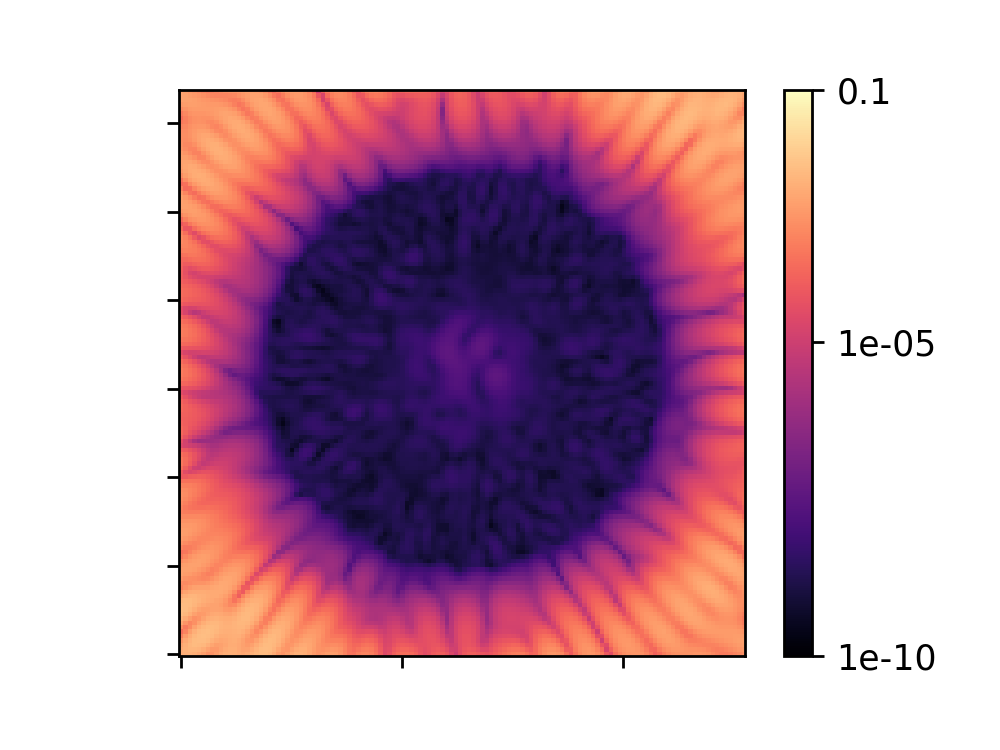
\includegraphics[width=0.51\textwidth]{0PSF.png}
    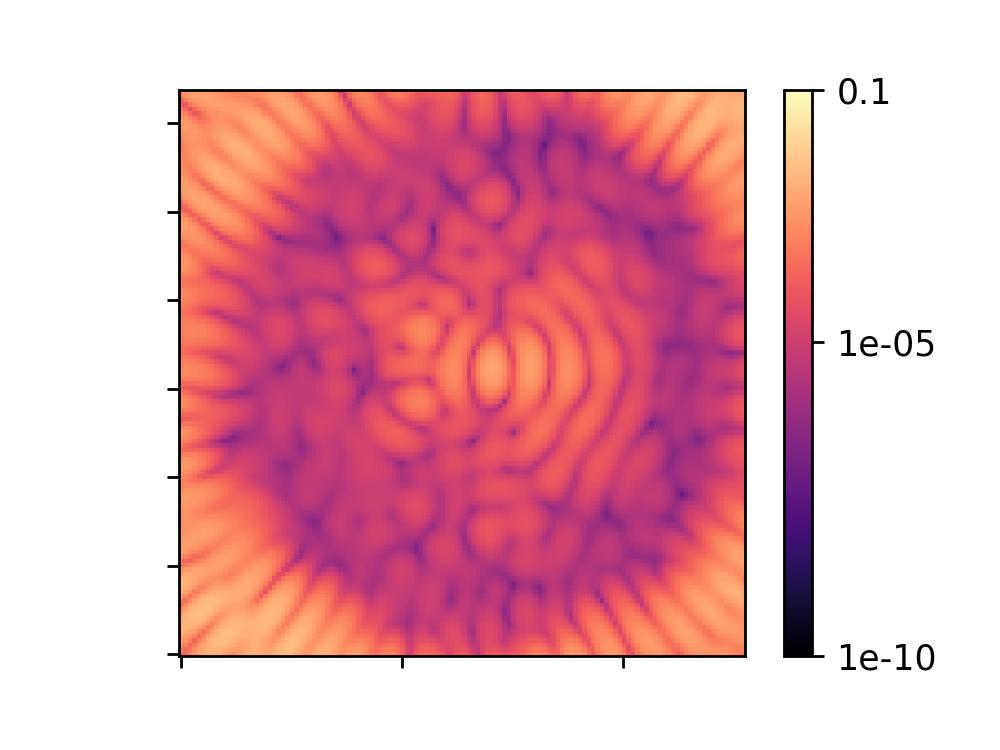
\includegraphics[width=0.49\textwidth]{17PSF_1lambdaD.png}
    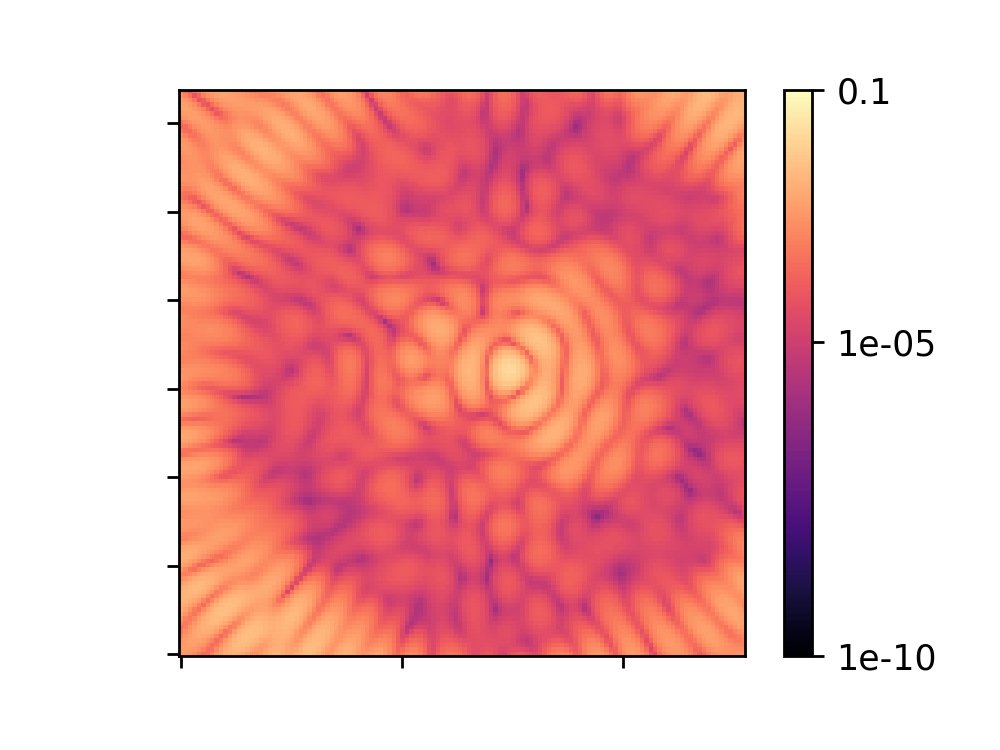
\includegraphics[width=0.49\textwidth]{34PSF_2lambdaD.png}
    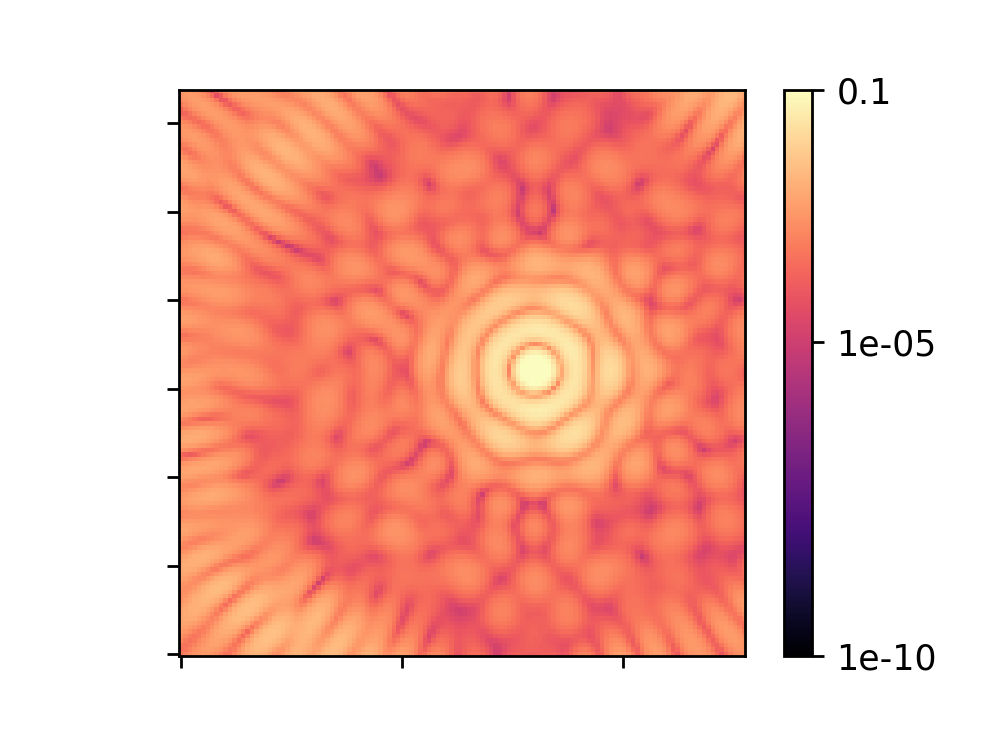
\includegraphics[width=0.49\textwidth]{51PSF.png}
    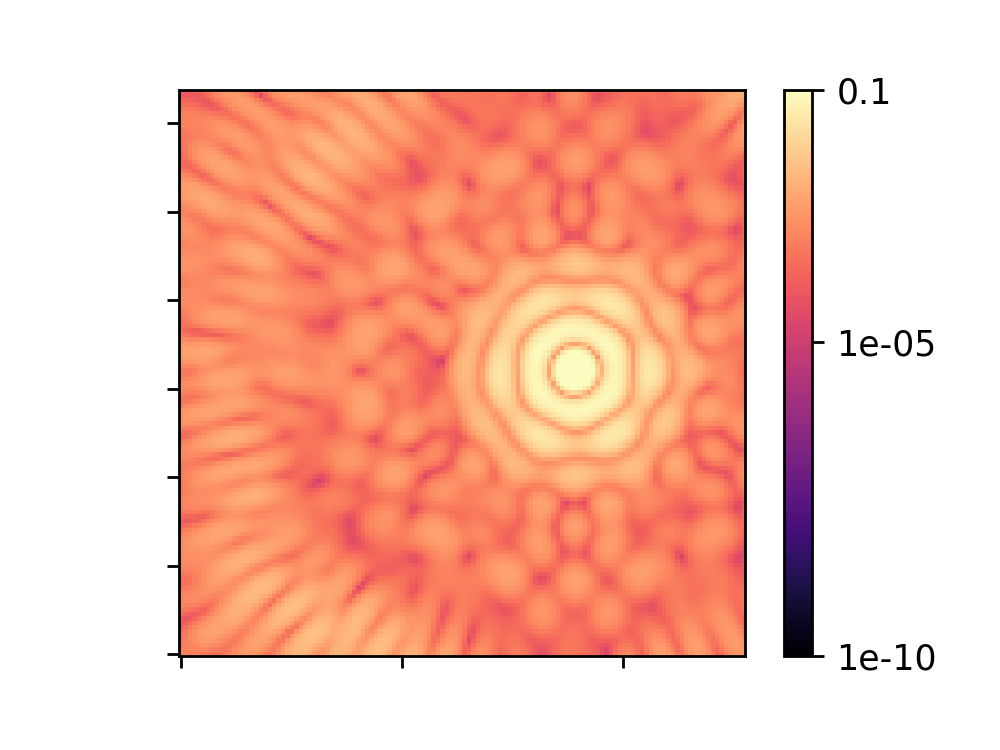
\includegraphics[width=0.49\textwidth]{68PSF.png}
    \caption{\acrshort{HLC} \gls{PSF} including transmission at a different separations. Top: On-axis coronagraph dark hole. Middle row: approx. 1 and 2$\lambda/D$ PSF. Significant flux is transmitted from sources inside the nominal 1.5$\lambda/D$ \acrshort{IWA}. Bottom row: approx. 3 and 4 $\lambda/D$ PSF. }
    \label{fig:psfs}
\end{figure}
\begin{figure}[!ht]
    \centering
    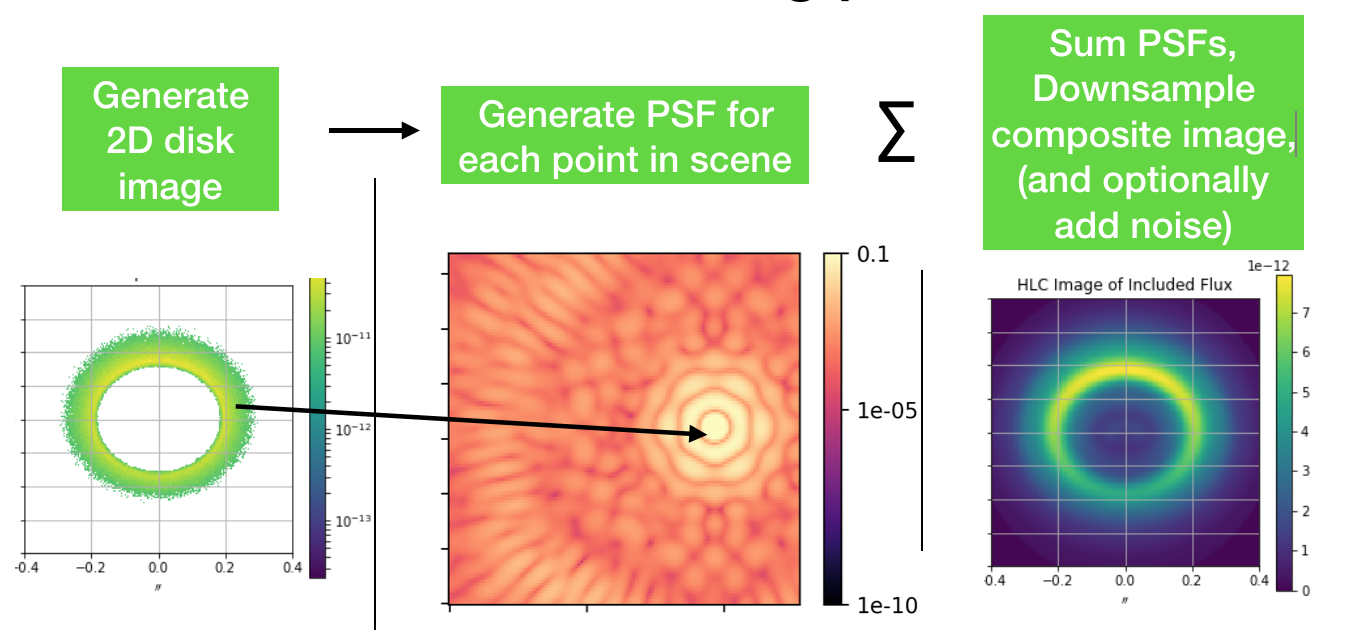
\includegraphics[width=0.95\textwidth]{flow.png}
    \caption{Simulation procedure for field dependant PSF simulations of circumstellar disks.}
    \label{fig:flow}
\end{figure}




\begin{figure}[!ht]
    \centering
    \caption{Exozodiacal dust simulations, using a Zodipic model of the solar system at 10 parsecs.
    The input sampling (left-most figures) is 3 mas/pixel and given in Jansky/pixel. Masked pixels are shown as unity and propagated values are zero in the mask map (central figures). The HLC model outputs (right-most figure) is sampled at 5 mas/pixel and have not been rebinned to the detector pixel. }\label{fig:zodi_models}
\begin{subfigure}{\textwidth}

    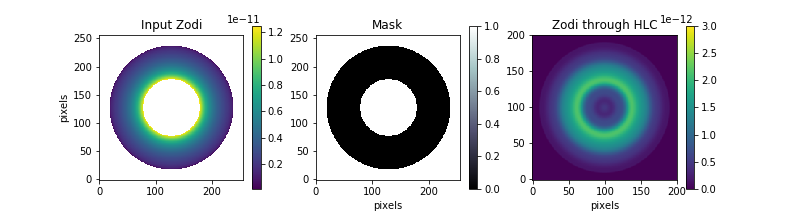
\includegraphics[width=0.95\textwidth]{masked_zodi.png}
    \caption{Exozodiacal dust simulation assuming all dust is outside the \gls{IWA} }
    \label{fig:mask}
    \end{subfigure}

\begin{subfigure}{\textwidth}
    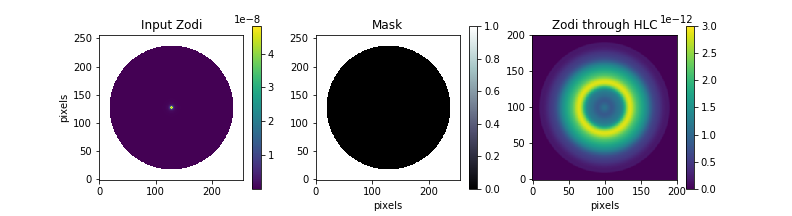
\includegraphics[width=0.95\textwidth]{unmasked_zodi.png}
    \caption{Including dust within the \acrshort{IWA} the disk brightens significantly, with the total flux transmitted increasing by approximately 25\%.}
    \label{fig:nomask}
    \end{subfigure}

\end{figure}


\section{Methods}
\label{sec:intro}  % \label{} allows reference to this section
Fig. \ref{fig:flow} shows our simulation procedure. 
We generate a simulated dust image in units of Jansky per pixel using Zodipic\cite{kuchner_zodipic_2012} or another simple optically-thin radiative transfer model.
Each pixel in the input scene is finely sampled, typically on a 3 mas grid.  
We build a composite image by multiplying the flux in the input pixel by the corresponding PSF array.
The PSF arrays are sampled from the 1D \gls{HLC} \gls{PSF} grid publicly shared on the IPAC WFIRST  website\footnote{http://wfirst.ipac.caltech.edu}.
Rotational symmetry is assumed and interpolation is  nearest neighbor since the \gls{PSF} grid is finely sampled.

\section{Preliminary Results}

    %to do: write ipynb DOI
    %fix bib
    %state that the disk brightens by >10%
    % summarize future plans
    Fig. \ref{fig:zodi_models} shows the effect of including flux inside the \gls{IWA} on the simulated dust.
    Fig. \ref{fig:mask} shows a the Zodipic Model truncated at approximately the \gls{CGI} \gls{IWA} (0.15 arcsec). The left panel shows the input flux used to simulate the image. The middle panel shows just the input pixels for clarity. 
    The resulting simulated image, accounting for \gls{HLC} throughput and \gls{PSF} morphology is shown in the right panel.
    Fig. \ref{fig:nomask} shows the same input model without an interior mask.
    A \gls{PSF} was generated for every unmasked point (shown as zero values in the mask or colored values in the input map).    The  total transmitted increases from Fig. \ref{fig:mask} to Fig. \ref{fig:nomask} by about 25\%.
    
    \section{Discussion}
    This early work shows scattered light from circumstellar disks inside the \gls{IWA} may impact the flux levels at larger separations, inside the dark hole where the stellar leakage is small.
    This provides an opportunity to better characterize exozodiacal dust and debris disks at small angular separations.
    Additionally, since flux is diffracted to large separations, dust scattered light inside the \gls{WFIRST} CGI \gls{IWA} may increase the background flux observed
    Particularly notable in Fig. \ref{fig:nomask}, for this circularly symmetric, face-on model,  is the brightening of the central point where the parent star will appear, which must be accounted for in flux calibration and \gls{PSF} subtraction.
    Future work is necessary to quantify the impact on post-processing and assess sensitivity to dust as a function of stellar type and distance as well as disk morphology and composition.
    
    A Jupyter notebook reproducing Fig. \ref{fig:zodi_models} is available from Github\footnote{\url{https://github.com/uasal/2019_ProcSPIE_WFIRST_CGI_Exozodi}} and citable in Zenodo\cite{douglas_douglase/2019_procspie_wfirst_cgi_exozodi_2019}. 
    The HLC PSF library is available from IPAC\footnote{\url{https://wfirst.ipac.caltech.edu/sims/off_axis_PSF.html}}.
        The presented simulations are computation limited since each input pixel's PSF is interpolated and rotated to the correct field position. Work is underway to eliminate this bottleneck by generation of a pre-interpolated, high-resolution grid of PSF's which can be directly applied to an input field array.

\acknowledgments % equivalent to \section*{ACKNOWLEDGMENTS}   


The authors acknowledge valuable inputs from  Vanessa Bailey,  Brian Kern, John Krist, Hanying Zhou,   and the rest of the JPL CGI team.
Portions of this work were supported by the WFIRST Science Investigation team prime award \#NNG16PJ24C.
Portions of this work were supported by the Arizona Board of Regents Technology Research
Initiative Fund (TRIF).
This research made use of the \gls{MGHPCC} via MIT Research Computing and High Performance Computing (HPC) resources supported by the University of Arizona (UA) TRIF, UITS, and RDI and maintained by the UA Research Technologies department.


This research made use of community-developed core Python packages, including: Astropy\cite{the_astropy_collaboration_astropy_2013}, Matplotlib\cite{hunter_matplotlib_2007}, SciPy\cite{jones_scipy_2001}, 
the IPython Interactive Computing architecture \cite{perez_ipython_2007}, and Jupyter\cite{kluyver_jupyter_2016}.
% References
\bibliography{wfirst} % bibliography data in report.bib
\bibliographystyle{spiebib} % makes bibtex use spiebib.bst

\end{document} 
